% =====================================================================
% MOSPACE -- proposed restructured version for CCGrid (v2)
% Built from IEEE-conference-template-062824.tex (commit 9ccca1d).
% Red [TODO: ...] notes are questions for the authors; hide them all by
% replacing \providecommand{\revnote} below with \newcommand{\revnote}[1]{}.
% =====================================================================
\documentclass[conference]{IEEEtran}
\IEEEoverridecommandlockouts
\usepackage{multirow}
\usepackage{booktabs}
\usepackage{cite}
\usepackage{amsmath,amssymb,amsfonts}
\usepackage{graphicx}
\usepackage{textcomp}
\usepackage{xcolor}
\usepackage{tabularx}
\usepackage{pgfplots}
\pgfplotsset{compat=1.18}
\usepgfplotslibrary{groupplots}
\usetikzlibrary{patterns}
\usepackage{tikz}
\usetikzlibrary{arrows.meta,fit,backgrounds}
\definecolor{archaccent}{RGB}{0,84,147}
\definecolor{archbroker}{RGB}{235,242,250}
\definecolor{archsite}{RGB}{244,244,244}
\definecolor{archcloud}{RGB}{253,243,230}
\definecolor{archcloudln}{RGB}{190,105,0}
\definecolor{archbusy}{RGB}{150,150,150}
\definecolor{archpred}{RGB}{233,245,233}
% \archpool{x}{y}{#busy of 5}{label}: a pool of identical on-premises nodes
\newcommand{\archpool}[4]{%
  \foreach \i in {0,...,4}{%
    \ifnum\i<#3\relax\def\archf{archbusy}\else\def\archf{white}\fi
    \draw[line width=0.4pt, fill=\archf] ({#1+\i*0.27},{#2}) rectangle ++(0.21,0.21);}
  \node[anchor=west, inner sep=1pt] at ({#1+1.36},{#2+0.105}) {#4};}
% \archvm{x}{y}{#running of 5}{label}: a cloud VM type; VMs exist only while used
\newcommand{\archvm}[4]{%
  \foreach \i in {0,...,4}{%
    \ifnum\i<#3\relax
      \draw[line width=0.4pt, draw=archcloudln, fill=archcloudln!45] ({#1+\i*0.27},{#2}) rectangle ++(0.21,0.21);
    \else
      \draw[line width=0.4pt, draw=archcloudln!70, dash pattern=on 1pt off 0.8pt] ({#1+\i*0.27},{#2}) rectangle ++(0.21,0.21);
    \fi}
  \node[anchor=west, inner sep=1pt] at ({#1+1.36},{#2+0.105}) {#4};}
% Author-facing notes; redefine as \newcommand{\revnote}[1]{} to hide them.
\providecommand{\revnote}[1]{{\color{red!70!black}\footnotesize[\textbf{TODO:} #1]}}


\begin{document}

\title{MOSPACE: Cost-Aware Scheduling of Parallel Jobs on a Federation of HPC Clusters and Cloud Resources
\thanks{Identify applicable funding agency here. If none, delete this.}
}

\author{\IEEEauthorblockN{1\textsuperscript{st} Bernardo Gallo}
\IEEEauthorblockA{\textit{Institute of Computing} \\
\textit{Universidade Federal Fluminense}\\
Niterói, Brazil\\
bgallo@id.uff.br}
\and
\IEEEauthorblockN{2\textsuperscript{nd} Lucia Drummond}
\IEEEauthorblockA{\textit{Institute of Computing} \\
\textit{Universidade Federal Fluminense}\\
Niterói, Brazil \\
lucia@ic.uff.br}
\and
\IEEEauthorblockN{3\textsuperscript{rd} José Viterbo}
\IEEEauthorblockA{\textit{Institute of Computing} \\
\textit{Universidade Federal Fluminense}\\
Niterói, Brazil\\
viterbo@ic.uff.br}
\and
\IEEEauthorblockN{4\textsuperscript{th} Eduardo Uchoa}
\IEEEauthorblockA{\textit{Department of Production Engineering} \\
\textit{Universidade Federal Fluminense}\\
Niterói, Brazil \\
uchoa@producao.uff.br}
}

\maketitle

\begin{abstract}
HPC centers size their clusters for the expected load, so demand peaks turn into long queues. Federating several clusters and bursting into public clouds adds capacity, but the scheduler must then decide where and when every job runs, trading job turnaround against the money spent on cloud instances and data transfers. Production resource managers such as Slurm route jobs across clusters by earliest expected start and ignore cost. We present MOSPACE, a central scheduler for a federation of on-premises clusters and on-demand cloud instance pools. At every submission and resource-release event, MOSPACE re-plans all jobs that have not started, minimizing a weighted combination of priority-weighted turnaround and monetary cost under bounded capacity, data-staging times and egress prices. Plans are computed by an arc-flow mixed-integer linear program (MILP) or, without a commercial solver, by a memetic genetic algorithm (GA). We evaluate MOSPACE in Batsim simulations of a production cluster of 1,654 nodes and 76,912 cores, driven by its Slurm accounting logs, with access to 12 AWS EC2 instance types. Without cloud offloading, MOSPACE lowers the mean waiting time by 20--49\% and the mean bounded slowdown by 43--76\% relative to the multi-cluster and federated modes of Slurm on three workloads. With offloading, on a four-hour congestion episode of 3,349 jobs, it keeps the mean waiting time at 1 minute for \$6.5k, while the Slurm configurations spend more than \$11k and still wait 8 minutes on average. On 108 benchmark instances, the MILP is solved to optimality in 91\,s on average and the GA stays within 4.4\% of the optimum in under 6\,s.
\end{abstract}

\begin{IEEEkeywords}
Federated HPC, cloud bursting, parallel job scheduling, cost-aware scheduling, multi-objective optimization.
\end{IEEEkeywords}

% =====================================================================
\section{Introduction}
% =====================================================================

On-premises HPC systems are finite. Their acquisition requires substantial capital investment, and their operation adds energy, cooling, maintenance and staff costs. Provisioning enough hardware for occasional demand peaks is economically inefficient, so HPC centers are designed around an expected workload. Periods of high demand therefore produce long queues and delay the users' work. Two complementary answers have emerged. \emph{Federated HPC} coordinates independently operated infrastructures through common services for access, resource allocation and data management~\cite{Foster2001,Gentzsch2011,Alam2022,Magugliani2025}, so that idle capacity at one site can absorb load from another. \emph{Cloud bursting} leases public-cloud virtual machines while the local system is congested~\cite{BUYYA2009599,mell2011nist,deAssuncao2009,Marshall2010}. Combining both yields a federation of fixed-capacity, free-at-the-margin clusters and elastic but priced cloud pools that differ in node types, provisioning delays, data-transfer times and egress prices.

Scheduling in such a federation is no longer only a question of \emph{when} a job starts, but also of \emph{where}: on which cluster, on which node type, or on which cloud instance type. Every placement trades turnaround against expenditure. Sending a job to the cloud shortens its wait but costs money; keeping it at home is free but may leave it queued for hours. Production resource and job management systems (RJMS) do not address this trade-off. Slurm, the most widely deployed RJMS~\cite{Yoo2003}, offers a multi-cluster mode that submits each job to the cluster with the earliest expected start and a federated mode that replicates jobs across member clusters~\cite{Jette2023}. Neither mode weighs monetary cost, and both decide one job at a time.

This paper presents MOSPACE, a central, cost-aware scheduler for a cloud-enabled HPC federation. MOSPACE keeps a global view of the queue, of the running jobs and of the free capacity of every resource pool. At every job submission and every resource release, it re-plans all jobs that have not started yet, choosing for each one an instance type and a start time. The plan minimizes a weighted combination of priority-weighted turnaround and monetary cost, subject to the capacity of each pool, the release time of each job and the time and price of moving its data between sites. A single weight $\lambda$ lets the center operator choose a point on the turnaround--cost trade-off. Plans are computed by an exact arc-flow mixed-integer linear program (MILP) solved with Gurobi~\cite{gurobi} or, when a commercial solver is not available, by a memetic genetic algorithm (GA) that returns near-optimal plans in seconds.

We evaluate MOSPACE with production data from Petrobras, the Brazilian energy company: the platform of an HPC cluster dedicated to reservoir simulation (1,654 nodes, 76,912 cores) and two workloads extracted from its Slurm accounting log, extended with 12 AWS EC2 on-demand instance types. The simulations use Batsim~\cite{batsim_jsspp16} and compare MOSPACE with FCFS, EASY backfilling and the multi-cluster and federated modes of Slurm. The main contributions are:
\begin{itemize}
  \item the design of MOSPACE, an event-driven, rolling-horizon scheduler that jointly decides placement and start time of parallel jobs across on-premises clusters and cloud instance pools, accounting for capacity, data staging and monetary cost;
  \item an arc-flow MILP formulation of the underlying planning problem, in which each homogeneous resource pool is a single flow graph, together with a memetic GA that exploits the zero marginal cost of on-premises execution;
  \item a trace-driven evaluation on a production platform and workloads, showing that MOSPACE dominates the cost--waiting-time trade-off achieved by Slurm's multi-cluster and federated modes, and a benchmark on 108 instances quantifying the speed and quality of both planners.
\end{itemize}

Section~\ref{sec:related_work} reviews related work. Section~\ref{sec:system} describes the architecture and online operation of MOSPACE. Section~\ref{sec:model} presents the planning model and Section~\ref{sec:ga} the GA. Section~\ref{sec:experimental_setup} describes the experimental setup, Section~\ref{sec:results} discusses the results and Section~\ref{sec:conclusion} concludes.

% =====================================================================
\section{Related Work}
\label{sec:related_work}
% =====================================================================

\emph{Federated and multi-site HPC.}
Parallel job scheduling on HPC systems has a long history~\cite{Feitelson2005}. Grid computing introduced the coordination of resources across administrative domains~\cite{Foster2001}, and infrastructures such as DEISA~\cite{Gentzsch2011} and Fenix~\cite{Alam2022} federate European supercomputing and cloud services~\cite{Haus2022}. At the scheduling layer, Sabin et al.~\cite{Sabin2003} studied the placement of parallel jobs across heterogeneous sites, Leal et al.~\cite{Leal2009} proposed a decentralized model for scheduling independent tasks in federated grids, and Wu et al.~\cite{Wu2025} survey task scheduling in geo-distributed computing. Wang et al.~\cite{Wang2025Efficient} propose a two-level architecture for heterogeneous clusters in which a global layer filters and scores clusters on capacity, affinity and estimated startup and data-transfer latency. Production RJMS offer simpler mechanisms: Slurm's multi-cluster mode sends each job to the cluster with the earliest expected start, and its federated mode replicates the job across member clusters, whose local schedulers coordinate so that it runs only once~\cite{Yoo2003,Jette2023}. These approaches are heuristic, decide one job at a time and ignore monetary cost. MOSPACE instead optimizes the placement of all pending jobs jointly against a common turnaround and cost objective.

\emph{Cloud bursting for HPC.}
De Assun\c{c}\~ao et al.~\cite{deAssuncao2009} evaluated the cost-benefit of extending cluster capacity with cloud resources, and Marshall et al.~\cite{Marshall2010} built Elastic Site, which extends a cluster managed by a local resource manager such as Torque with cloud nodes provisioned according to demand. Mateescu et al.~\cite{Mateescu2011} propose a hybrid HPC architecture that spans resources with different owners, policies and locations. Kailasam et al.~\cite{kailasam2010} proposed autonomic cloud-bursting schedulers with probabilistic service-level guarantees for data-intensive workloads, and Lilienthal~\cite{Lilienthal2013} proposed an economic model to size the internal capacity used with cloud bursting. Closer to our setting, Ambati et al. analyzed how much fixed capacity a cloud-enabled scheduler should provision~\cite{ambati2020waiting} and policies that trade job waiting against cloud expenditure~\cite{ambati2021good}, and Starburst~\cite{Luo24} adjusts waiting budgets over private and cloud clusters to improve the cost--turnaround trade-off. These works rely on threshold or waiting policies; none plans start times and placements jointly over several heterogeneous, capacity-bounded pools with data-staging costs.

\emph{Optimization models.}
Mathematical scheduling models cover parts of the problem. Brotcorne et al.~\cite{Brotcorne2023} minimize makespan and cost for bags of identical tasks on capacity-constrained multi-cloud platforms, without release times. Kramer et al.~\cite{Kramer2020} minimize weighted completion time with release dates on identical parallel machines with arc-flow formulations, without costs. Chen et al.~\cite{Chen2024} handle unrelated machines with machine-usage costs, but all jobs are available at time zero, which makes scheduling within one machine polynomial. Table~\ref{tab:literature} summarizes the comparison: MOSPACE is, to our knowledge, the first to combine release times, monetary cost, data movement and bounded hybrid pools in an online scheduler evaluated against production RJMS.

\begin{table}[t]
\centering\footnotesize
\setlength{\tabcolsep}{3pt}
\caption{Comparison with the closest works.}
\label{tab:literature}
\setlength{\tabcolsep}{2pt}
\begin{tabular}{lccccl}
\toprule
Work & Release & Cost & Data & Online & Environment \\
\midrule
Slurm multi-cl./fed.~\cite{Jette2023} & yes & no & no & yes & federated HPC \\
Wang et al.~\cite{Wang2025Efficient} & no & no & yes & yes & federated \\
Starburst~\cite{Luo24} & yes & yes & no & yes & hybrid \\
Brotcorne et al.~\cite{Brotcorne2023} & no & yes & no & no & multi-cloud \\
Kramer et al.~\cite{Kramer2020} & yes & no & no & no & on-premises \\
Chen et al.~\cite{Chen2024} & no & yes & no & no & unrelated machines \\
\textbf{MOSPACE} & yes & yes & yes & yes & federated + cloud \\
\bottomrule
\end{tabular}
\end{table}
\revnote{Check the Release and Online columns for Wang et al.; Starburst schedules jobs arriving over time (USENIX abstract), so Release is now ``yes''. The original table.tex had no Online column.}

% =====================================================================
\section{MOSPACE Architecture}
\label{sec:system}
% =====================================================================

\begin{figure}[t]
\centering
\includegraphics[width=\columnwidth]{figures/architecture.pdf}
\caption{MOSPACE in a cloud-enabled Slurm federation. MOSPACE, at the federation level, decides where (pool $\hat m_j$) and when (start $\hat t_j$) each pending job runs, using predicted runtimes and I/O volumes; the Slurm instance of each member cluster executes these decisions: it allocates and launches the job, stages its data, resumes and suspends cloud VMs, and reports events and accounting back. Each on-premises pool is a set of identical nodes at one site (gray: busy); each cloud pool is one VM type, whose instances exist only while they run a job. Green: predictors, replaced in our evaluation by the runtimes and data volumes recorded for the jobs.}
\label{fig:architecture}
\end{figure}

MOSPACE is a central scheduler placed above the resource pools of the federation (Fig.~\ref{fig:architecture}). A \emph{resource pool} is a set of homogeneous instances of one \emph{instance type} at one site: a node group of an on-premises cluster, or a VM type of a cloud region. On-premises pools have fixed capacity and no marginal cost. Cloud pools are elastic and priced per instance and per unit of time. Each job is a non-preemptive parallel job that requests a number of nodes of a node type, as in an \texttt{sbatch} submission; it may run on any pool whose instances satisfy its CPU, memory, storage and GPU requirements and that lies at a site the job is allowed to use. A job runs on instances of a single pool and does not span sites. Its input data reside at an origin site and its results must be returned there, so running it elsewhere adds staging time and possibly egress charges.

MOSPACE and Slurm split the work. MOSPACE decides \emph{where} and \emph{when} every pending job runs; the Slurm controller of each member cluster, including a cloud cluster whose nodes are VMs resumed and suspended on demand, decides nothing about placement and only \emph{executes} the plan: it allocates nodes, launches and confines the job, stages its data in and out, and records accounting. MOSPACE has six components. The \emph{job queue} holds the jobs that have been submitted but not started. The \emph{runtime predictor} and the \emph{I/O predictor} estimate, from the accounting history of past jobs, the execution time and the input and output data volumes of each job, which determine its occupation, staging time and egress cost on every pool. The \emph{state monitor} tracks running jobs, the free capacity of every pool and cloud prices from the events reported by Slurm. The \emph{planner} computes a plan, i.e., a pool and a start time for every job in the queue. The \emph{dispatcher} submits each job to the Slurm cluster of its planned pool when its planned start time is reached.

\emph{Online operation.} MOSPACE works in a rolling-horizon fashion. Every job submission and every resource release (a job completion) triggers a new planning round. The planner receives the current state: running jobs keep their instances until their expected completion, and every job that has not started, including those already planned in previous rounds, can be rescheduled to any compatible pool and start time. The planner returns a new plan for the whole queue, and the dispatcher follows it until the next event. Re-planning all pending jobs at every event keeps the plan consistent with the actual system state, so early completions are exploited immediately and newly arrived jobs can take capacity that was reserved for jobs with a better cloud alternative. In our deployment, the MILP planner runs with a time limit of 180\,s per round and usually finishes in about one minute; the GA answers in seconds. \revnote{How is the planner time accounted for in the simulation (is the simulated clock frozen during a round, or are rounds started at most once per interval / batched)? W1 has a submission every $\approx$7\,s on average. Also give the horizon length $H$ and step $\Delta$ used online, and whether data movement is modeled in the online runs.}

\emph{Runtime knowledge.} Like backfilling schedulers, MOSPACE needs runtime estimates. Our evaluation uses the runtimes recorded in the traces. User-provided estimates are known to be inaccurate~\cite{Mualem2001}, but system-generated predictions improve them~\cite{Tsafrir2007}, and for the cluster studied here a two-step machine-learning estimator has been proposed to predict the runtime interval of reservoir-simulation jobs~\cite{Nunes2025}. Since MOSPACE re-plans at every completion, estimation errors are partially corrected as soon as a job finishes earlier than predicted.

% =====================================================================
\section{Planning Model}
\label{sec:model}
% =====================================================================

At each planning round, the planner solves the following problem for the set of pending jobs.

\subsection{Resources, jobs and data}

Let $J=\{1,\ldots,n\}$ be the jobs, $\mathcal{S}$ the sites (on-premises clusters and cloud regions) and $M=M^{\mathrm{on}}\cup M^{\mathrm{cloud}}$ the instance types. Type $m$ is located at site $\sigma(m)$, has at most $N_m$ instances, per-instance capacities $C_m^r$ for $r\in R=\{\mathrm{cpu},\mathrm{mem},\mathrm{stor},\mathrm{gpu}\}$, a performance factor $P_m>0$ and a provisioning time $\pi_m^{\mathrm{raw}}$. For a cloud type, any $N_m\geq\sum_j q_j$ makes the bound non-binding. The horizon is discretized as $T=\{0,\ldots,H\}$ with step $\Delta$.

Job $j$ arrives at $a_j\in T$, has base execution time $e_j^{\mathrm{raw}}$, priority weight $w_j\geq0$, node count $q_j$, per-instance demands $q_j^r$ and allowed sites $\mathcal{S}_j$. Its feasible types are $F_j=\{m\in M: q_j^r\leq C_m^r\ \forall r,\ q_j\leq N_m,\ \sigma(m)\in\mathcal{S}_j\}$. Its input data, of volume $\iota_j^{\mathrm{in}}$, reside at site $o_j$, and its results, of volume $\iota_j^{\mathrm{out}}$, must reach site $d_j$ (usually $d_j=o_j$). A link between sites $s$ and $s'$ has transfer time $\theta_{ss'}^{\mathrm{raw}}$ and price $\kappa_{ss'}$ per volume unit, both zero when $s=s'$; typically $\kappa_{ss'}>0$ only for internet egress from a cloud region. Running job $j$ on type $m$ therefore requires the transfer time and price
\begin{align}
 \tau_{jm}^{\mathrm{raw}}&=\theta_{o_j\sigma(m)}^{\mathrm{raw}}\iota_j^{\mathrm{in}}+\theta_{\sigma(m)d_j}^{\mathrm{raw}}\iota_j^{\mathrm{out}},\\
 \kappa_{jm}^{\mathrm{IO}}&=\kappa_{o_j\sigma(m)}\iota_j^{\mathrm{in}}+\kappa_{\sigma(m)d_j}\iota_j^{\mathrm{out}}.
\end{align}

\subsection{Durations and costs}

Staging holds the instances, so the billable duration of $j$ on $m$, in steps, is $p_{jm}^{\mathrm{bill}}=\max\{1,\lceil(e_j^{\mathrm{raw}}/P_m+\tau_{jm}^{\mathrm{raw}})/\Delta\rceil\}$. Provisioning also holds the instances but is not billed, so the occupation is $p_{jm}^{\mathrm{occ}}=p_{jm}^{\mathrm{bill}}+\lceil\pi_m^{\mathrm{raw}}/\Delta\rceil$. With $\kappa_m^{\mathrm{VM}}$ and $\kappa_m^{\mathrm{S}}$ the per-instance prices of use and of allocated storage per unit of time, both zero on premises, the cost of the job is
\begin{equation}
 c_{jm}=\kappa_{jm}^{\mathrm{IO}}+q_j(\kappa_m^{\mathrm{VM}}+\kappa_m^{\mathrm{S}}q_j^{\mathrm{stor}})\,p_{jm}^{\mathrm{bill}}\Delta,
\end{equation}
which models billing in blocks of $\Delta$ with a minimum of one block. A remote pool is thus simply a slower, and possibly priced, option for the job. The feasible starts are $T_{jm}=\{t\in T:t\geq a_j,\ t+p_{jm}^{\mathrm{occ}}\leq H\}$.

\subsection{Arc-flow formulation}

Each type $m$ has a directed acyclic graph $G_m=(T,A_m)$ whose nodes are the time steps. Waiting arcs $(t,t+1)$ represent idle instances, and processing arcs $(j,t,t+p_{jm}^{\mathrm{occ}})$, for $j$ with $m\in F_j$ and $t\in T_{jm}$, represent job $j$ holding $q_j$ instances of $m$ over $[t,t+p_{jm}^{\mathrm{occ}})$. Binary $x_{jmt}$ selects a processing arc and $y_{mt}$ is the number of idle instances of $m$ during $[t,t+1)$, with $y_{m,-1}=y_{m,H}=N_m$. The constraints are
\begin{align}
&\textstyle\sum_{m\in F_j}\sum_{t\in T_{jm}}x_{jmt}=1 && \forall j\in J, \label{eq:model-assignment}\\
&\begin{aligned}
y_{m,v-1}&+\textstyle\sum_{j:\,v-p_{jm}^{\mathrm{occ}}\in T_{jm}} q_j x_{jm,v-p_{jm}^{\mathrm{occ}}}\\
&=y_{mv}+\textstyle\sum_{j:\,v\in T_{jm}} q_j x_{jmv}
\end{aligned} && \forall m\in M,\ v\in T, \label{eq:model-flow}\\
&x_{jmt}\in\{0,1\},\quad 0\leq y_{mt}\leq N_m. \nonumber
\end{align}
Constraint~\eqref{eq:model-assignment} gives each job one pool and one start, and~\eqref{eq:model-flow} conserves the $N_m$ units of flow of each pool: a job takes $q_j$ instances when it starts and returns them when it ends. Summing~\eqref{eq:model-flow} over time shows that $y_{mu}\geq0$ is exactly the requirement that overlapping jobs never use more than $N_m$ instances, and that $y$ is integral whenever $x$ is. A whole pool of identical nodes is therefore one graph, regardless of its size, and node-level assignment is left to the local RJMS. In the online setting, running jobs reduce the available capacity of their pool until their expected completion.

\subsection{Objectives and scalarization}

The two objectives are the priority-weighted turnaround and the monetary cost,
\begin{equation}
 f_1=\sum_{j,m,t} w_j\,(t+p_{jm}^{\mathrm{occ}}-a_j)\,x_{jmt},\qquad
 f_2=\sum_{j,m,t} c_{jm}\,x_{jmt}.
\end{equation}
Because they have different units, we normalize them by the lexicographic extremes of the feasible set: the time-first solution $(f_1^{\mathrm{lex}},f_2^{\mathrm{lex}})$, which minimizes $f_1$ and then $f_2$, and the cost-first solution $(f_1^{0},f_2^{0})$, which minimizes $f_2$ and then $f_1$. With $\widehat f_1=(f_1-f_1^{\mathrm{lex}})/(f_1^0-f_1^{\mathrm{lex}})$ and $\widehat f_2=(f_2-f_2^0)/(f_2^{\mathrm{lex}}-f_2^0)$, the planner solves
\begin{equation}
\label{eq:scalarization}
\min\ \lambda\widehat f_1+(1-\lambda)\widehat f_2\quad\text{s.t.}\ \eqref{eq:model-assignment}\text{--}\eqref{eq:model-flow},\ f_1\leq f_1^0,
\end{equation}
for an operator-chosen $\lambda\in[0,1]$; larger values favor turnaround. The cap $f_1\leq f_1^0$ discards only schedules dominated by the cost-first solution, so every Pareto-optimal point remains reachable. If the two extremes coincide, one schedule minimizes both objectives and no normalization is needed.

\subsection{Illustrative example}
\label{sec:example}

\begin{figure}[t]
\centering
\resizebox{\columnwidth}{!}{%
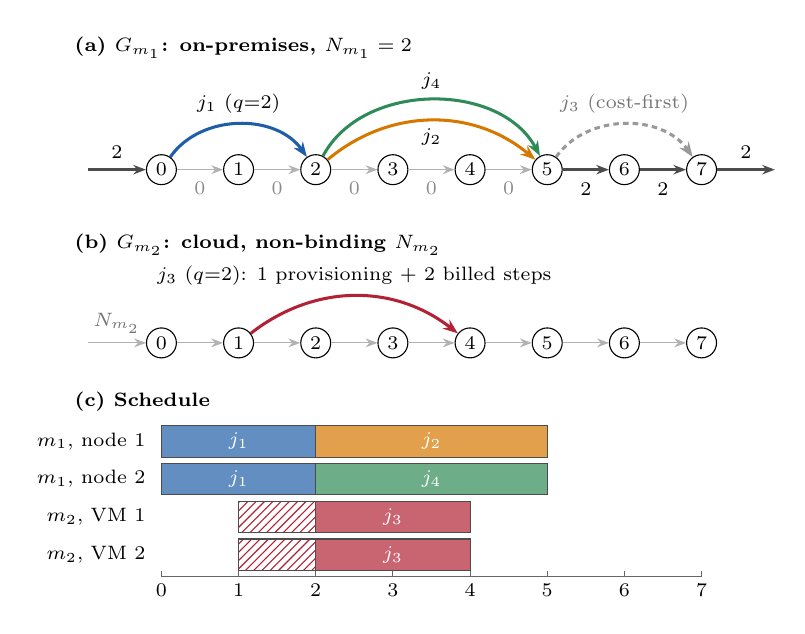
\begin{tikzpicture}[x=0.98cm, y=1cm, font=\scriptsize,
  tn/.style={circle, draw, inner sep=0pt, minimum size=3.8mm, fill=white},
  wa/.style={->, >={Stealth[length=1.5mm]}, line width=0.4pt, draw=black!30},
  wf/.style={->, >={Stealth[length=1.6mm]}, line width=1.3pt, draw=black!70},
  pa/.style={->, >={Stealth[length=1.9mm]}, line width=1.1pt},
  bar/.style={draw=black!70, line width=0.4pt},
]
\definecolor{jA}{RGB}{31,94,166}\definecolor{jB}{RGB}{214,120,0}
\definecolor{jC}{RGB}{178,34,52}\definecolor{jD}{RGB}{46,139,87}
% ---------------- (a) on-premises graph
\node[anchor=west, font=\scriptsize\bfseries] at (-1.25,1.55) {(a) $G_{m_1}$: on-premises, $N_{m_1}=2$};
\foreach \t in {0,...,7} \node[tn] (a\t) at (\t,0) {\t};
\foreach \t/\f in {0/0,1/0,2/0,3/0,4/0,5/2,6/2}{%
  \pgfmathtruncatemacro{\n}{\t+1}%
  \ifnum\f>0 \draw[wf] (a\t) -- (a\n) node[midway, below=1pt] {\f};
  \else \draw[wa] (a\t) -- (a\n) node[midway, below=1pt, text=black!45] {0}; \fi}
\draw[wf] (-0.95,0) -- node[above] {2} (a0);
\draw[wf] (a7) -- node[above] {2} (7.95,0);
\draw[pa, draw=jA] (a0) to[bend left=55] node[above] {$j_1$ ($q{=}2$)} (a2);
\draw[pa, draw=jB] (a2) to[bend left=40] node[pos=0.5, below=-1pt] {$j_2$} (a5);
\draw[pa, draw=jD] (a2) to[bend left=62] node[above] {$j_4$} (a5);
\draw[pa, draw=black!40, dash pattern=on 2pt off 1.5pt] (a5) to[bend left=55]
  node[above, text=black!55] {$j_3$ (cost-first)} (a7);
% ---------------- (b) cloud graph
\node[anchor=west, font=\scriptsize\bfseries] at (-1.25,-0.95) {(b) $G_{m_2}$: cloud, non-binding $N_{m_2}$};
\foreach \t in {0,...,7} \node[tn] (b\t) at (\t,-2.2) {\t};
\foreach \t in {0,...,6}{\pgfmathtruncatemacro{\n}{\t+1}\draw[wa] (b\t) -- (b\n);}
\draw[wa] (-0.95,-2.2) -- node[above, text=black!55] {$N_{m_2}$} (b0);
\draw[pa, draw=jC] (b1) to[bend left=38] node[above, align=center]
  {$j_3$ ($q{=}2$): 1 provisioning + 2 billed steps} (b4);
% ---------------- (c) schedule
\node[anchor=west, font=\scriptsize\bfseries] at (-1.25,-2.95) {(c) Schedule};
\foreach \r/\lab in {0/{$m_1$, node 1},1/{$m_1$, node 2},2/{$m_2$, VM 1},3/{$m_2$, VM 2}}
  \node[anchor=east] at (-0.08,{-3.45-0.48*\r}) {\lab};
\foreach \r in {0,1} \filldraw[bar, fill=jA!70] (0,{-3.65-0.48*\r}) rectangle (2,{-3.25-0.48*\r});
\filldraw[bar, fill=jB!70] (2,-3.65) rectangle (5,-3.25);
\filldraw[bar, fill=jD!70] (2,-4.13) rectangle (5,-3.73);
\foreach \r in {2,3}{%
  \filldraw[bar, pattern=north east lines, pattern color=jC] (1,{-3.65-0.48*\r}) rectangle (2,{-3.25-0.48*\r});
  \filldraw[bar, fill=jC!70] (2,{-3.65-0.48*\r}) rectangle (4,{-3.25-0.48*\r});}
\node[text=white] at (1,-3.45) {$j_1$}; \node[text=white] at (1,-3.93) {$j_1$};
\node[text=white] at (3.5,-3.45) {$j_2$}; \node[text=white] at (3.5,-3.93) {$j_4$};
\node[text=white] at (3,-4.41) {$j_3$}; \node[text=white] at (3,-4.89) {$j_3$};
\draw[black!60] (0,-5.17) -- (7,-5.17);
\foreach \t in {0,...,7}{\draw[black!60] (\t,-5.17) -- (\t,-5.10); \node[below=-1pt] at (\t,-5.17) {\t};}
\end{tikzpicture}}
\caption{Arc-flow solution of the example for $\lambda=0.5$. (a), (b): thick arcs carry flow (instances), with the idle flow $y_{mt}$ on the waiting arcs of $G_{m_1}$; the dashed arc is used by the cost-first solution. (c): a node assignment that realizes the flow; hatched: provisioning, not billed.}
\label{fig:example}
\end{figure}

Fig.~\ref{fig:example} shows the model on a small instance with one on-premises type $m_1$ of $N_{m_1}=2$ nodes and one cloud type $m_2$ that charges 1 per instance and step and needs one step of provisioning; there is no data transfer, $P_m=1$, $\Delta=1$ and $H=7$. Four jobs, given as $(a_j,e_j,q_j,w_j)$, must be planned: $j_1=(0,2,2,2)$, a high-priority two-node job; $j_2=(0,3,1,1)$; $j_3=(1,2,2,1)$, another two-node job; and $j_4=(2,3,1,1)$.

In the optimal plan for $\lambda=0.5$, the two units of flow of $G_{m_1}$ both enter the arc of $j_1$, which holds the two nodes during $[0,2)$. At node~2 they split between the arcs of $j_2$ and $j_4$, which have the same endpoints and are distinguished by their job index; the waiting arcs carry no flow ($y_{m_1t}=0$) until both units return at node~5 and stay idle until $H$. Job $j_3$ arrives at $t=1$, while $j_1$ holds both nodes; from $t=2$ on they are taken by $j_2$ and $j_4$, so $j_3$ could only start on premises at $t=5$. The plan sends it to the cloud: its arc in $G_{m_2}$ spans $[1,4)$, i.e., one step of provisioning, which occupies the instances but is not billed, followed by two billed steps on two instances. Job $j_2$ waits two steps on premises instead of being offloaded. The plan has $f_1=2\cdot2+5+3+3=15$ and $f_2=4$. For comparison, the time-first solution also offloads $j_2$, reaching $(f_1,f_2)=(14,7)$, and the cost-first solution keeps $j_3$ on premises in $[5,7)$ (dashed arc), reaching $(18,0)$. With the normalization of~\eqref{eq:scalarization}, the plan scores $0.5\cdot\frac{1}{4}+0.5\cdot\frac{4}{7}\approx0.41$ and is the unique optimum for $\lambda=0.5$; the instance has four Pareto-optimal points, $(14,7)$, $(15,4)$, $(16,3)$ and $(18,0)$. The model only decides how many instances of each pool a job holds and when: any decomposition of the flow of $G_{m_1}$ into paths gives a node assignment such as the one of Fig.~\ref{fig:example}(c), and in practice this assignment is left to the local RJMS.

% =====================================================================
\section{A Fast Planner: Memetic Genetic Algorithm}
\label{sec:ga}
% =====================================================================

The MILP needs a commercial solver for good performance and up to minutes per round. As an alternative planner, we designed a memetic algorithm~\cite{Moscato1989}, a GA whose offspring are improved by local search, which exploits a structural property of the problem: on-premises execution is free, so the cost $f_2$ depends only on \emph{which} jobs are sent to the cloud, and once that set is fixed, minimizing $f_1$ amounts to list scheduling on the bounded on-premises pools.

\emph{Representation and decoding.} A chromosome has one gene per job with three values: \emph{cloud} (run on the best cloud type, immediately), \emph{on-premises} (never offload), or \emph{auto} (offload only when waiting on premises becomes worse than the cloud). Start times and on-premises pools are not encoded; a constructive decoder derives them, so every individual yields a capacity-feasible schedule. Since both objectives are sums over jobs, each job has a score, its weighted contribution to~\eqref{eq:scalarization} at a given pool and start, which the decoder and the local search use to compare options. Three further genes select the decoder and evolve with the solution~\cite{Eiben1999}: a priority rule, either a weighted-shortest-processing-time index~\cite{Smith1956} biased toward jobs with an expensive cloud alternative or an earliest-deadline rule in which a job's deadline is the last start at which staying on premises still beats the cloud; whether jobs are offloaded when they pass that deadline; and a time-driven dispatch decoder or a serial schedule-generation scheme~\cite{Kolisch1996}.

\emph{Search.} Each new individual is improved by a hill climber that flips single job genes between cloud and on-premises; candidate moves are ranked by an $O(1)$ estimate of the score change, and only a short list is decoded exactly. Offspring are produced by multi-step crossover fusion~\cite{Yamada1996}, a guided walk from one parent toward the other, followed by mutation. The population is seeded with constructive heuristics, with two locally optimal all-\emph{auto} individuals and with random individuals; elitism keeps the best individual of each priority rule, and iterated-local-search kicks restart a stagnated search. Capacity and infeasibility are handled by penalties in the fitness. We use a population of 16 individuals and 120 generations. Offspring are generated in parallel with per-offspring random seeds, so results are deterministic for a fixed seed regardless of the number of threads. \revnote{Full GA details (penalties, rules, seeds, parameters) could go to a technical report or the code repository; add the link here.}

% =====================================================================
\section{Experimental Setup}
\label{sec:experimental_setup}
% =====================================================================

\subsection{Simulation platform and workloads}

The online experiments are simulated with Batsim~5~\cite{batsim_jsspp16}, a resource and job management simulator built on SimGrid~\cite{Casanova2014}. Batsim owns the clock, job submissions, job execution and the output traces, and delegates every scheduling decision to an external decision component that it queries over its protocol. We implemented MOSPACE and the baselines as such components, together with a wrapper that exports the platform and the workloads to Batsim's formats and collects the metrics.

The on-premises side is a production cluster of Petrobras dedicated to reservoir simulation. It is modeled from its Slurm node definitions as four homogeneous node groups of two-socket Intel Xeon nodes, $1{,}654$ nodes and $76{,}912$ cores in total; each node group is a member cluster (C1--C4) of the federation. The cloud side is one partition with the 12 AWS EC2 on-demand instance types of Table~\ref{tab:cloud}, priced at their us-east-1 Linux list prices. Each on-premises node type has a list of compatible cloud types with at least its physical core count and clock frequency and a CPU generation that is not older, and an offloaded job may only use the types compatible with the node type it requests. All types are assumed to run jobs at the speed of the on-premises nodes.

Both workloads come from the cluster's Slurm accounting log (Table~\ref{tab:workloads}). Each is cut at a time $t_0$. The \emph{initial-state jobs}, submitted before $t_0$, are running or pending at $t_0$; they always run on premises and form the load each strategy faces. The \emph{window jobs} are submitted during a window that starts at $t_0$, and only they may be offloaded. The simulation ends when the last job completes. Workload~1 (W1) is a submission burst of 1\,h\,48\,min on 25~November~2024, with single-node jobs shorter than 12\,h. Workload~2 (W2) is a four-hour congestion episode on 30~January~2024, larger and with a heavy runtime tail (174 jobs exceed 12\,h, the longest runs 496\,h). For the comparison without cloud, we also use 917 jobs from the public MIT Supercloud dataset~\cite{Samsi2021}. \revnote{Describe how the MIT Supercloud subset and its platform were built.}

\begin{table}[t]
  \centering\footnotesize
  \setlength{\tabcolsep}{4pt}
  \caption{Workloads. Statistics are over window jobs.}
  \label{tab:workloads}
  \begin{tabular}{lrr}
    \toprule
                                        & W1 (Nov.~2024) & W2 (Jan.~2024) \\
    \midrule
    Submission window                   & 1\,h\,48\,min & 4\,h \\
    Window jobs                         & 964        & 3{,}349 \\
    Initial-state jobs (run./pend.)     & 2{,}325 (1{,}932/393) & 3{,}215 (2{,}706/509) \\
    Window CPU-hours                    & 44{,}177   & 261{,}945 \\
    Runtime: median / mean              & 37\,min / 1.76\,h & 52\,min / 2.39\,h \\
    Runtime: P95 / max                  & 8.6\,h / 11.4\,h  & 12.3\,h / 495.6\,h \\
    Cores per job                       & 20, 40 or 64 & 4--64 (mean 24.5) \\
    Mean waiting time in the trace      & 36.8\,min  & 30.8\,min \\
    \bottomrule
  \end{tabular}
\end{table}

\begin{table}[t]
  \centering\footnotesize
  \setlength{\tabcolsep}{3pt}
  \caption{Cloud instance types (on-demand, AWS us-east-1).}
  \label{tab:cloud}
  \begin{tabular}{lrr@{\quad}lrr}
    \toprule
    Type & Cores & \$/h & Type & Cores & \$/h \\
    \midrule
    c6a.24xlarge & 48 & 3.67 & c6i.32xlarge & 64 & 5.44 \\
    c5a.24xlarge & 48 & 3.70 & m6i.32xlarge & 64 & 6.14 \\
    c5.24xlarge  & 48 & 4.08 & c7a.32xlarge & 64 & 6.57 \\
    c6i.24xlarge & 48 & 4.08 & r6i.32xlarge & 64 & 8.06 \\
    m5a.24xlarge & 48 & 4.13 & c7i.48xlarge & 96 & 8.57 \\
    m5.24xlarge  & 48 & 4.61 & c7a.48xlarge & 96 & 9.85 \\
    \bottomrule
  \end{tabular}
\end{table}

\subsection{Baselines and metrics}

We compare MOSPACE with four policies: FCFS; EASY backfilling~\cite{Lifka1995}; Slurm multi-cluster, which submits each job to the member cluster with the earliest expected start; and Slurm federated, which replicates each job on all eligible clusters and runs it on the first that can start it~\cite{Jette2023}. With cloud offloading, the Slurm baselines see the cloud as an additional member cluster of fixed size (50, 100, 200 or 400 nodes), and each offloaded job runs on the cheapest compatible VM type; MOSPACE has no such bound and is swept over $\lambda\in\{0.25,0.5,0.75\}$. \revnote{Confirm how the Slurm modes were emulated in Batsim (local policy of each member cluster: EASY?).} We report, for the window jobs, the turnaround and waiting times, the mean bounded slowdown $\max\{1,(w+r)/\max\{r,10\,\mathrm{s}\}\}$, where $w$ is the wait and $r$ the runtime, the number of offloaded jobs and the cloud cost.

\subsection{Benchmark instances}

To measure planner speed and quality in isolation, we generated 108 offline instances from the same job characteristics, in a full factorial over: two machine catalogues (Class~A: the two real node types of the cluster, 40 cores/300\,GB and 64 cores/480\,GB, each with one AWS equivalent; Class~B: four on-premises types, each with an AWS and an Azure equivalent); the two workloads; $N\in\{100,300,500\}$ nodes per on-premises type; an initial load of 0, $\lfloor N/2\rfloor$ or $N$ busy nodes per type; and three I/O levels. A cloud equivalent is the smallest instance of the same Intel generation (AWS m6i, Azure Dsv5, or D128s\_v6 for the 64-core node) whose physical cores and memory cover the on-premises node, priced at Linux on-demand list prices with unlimited capacity and $P_m=1$. All jobs originate on premises with no input staging; results return home through internet egress at \$0.09/GB (AWS) or \$0.08/GB (Azure), with transfer rates bound by the VM's disk throughput (7.63\,s/GB for AWS gp3, 8.0\,s/GB for Azure Premium SSD v2), so Azure is cheaper but slower to egress. \revnote{Give the data volumes of the I/O levels L/M/H.} Each instance is solved for $\lambda\in\{0.25,0.5,0.75\}$; the GA is run with 3 seeds.

% =====================================================================
\section{Results}
\label{sec:results}
% =====================================================================

\begin{table*}[t]
\centering
\small
\caption{Window jobs without cloud offloading. BSLD: mean bounded slowdown. Best value per workload in bold.}
\label{tab:no-cloud-slurm-baselines}
\resizebox{\textwidth}{!}{%
\begin{tabular}{lrrrrrrrr}
\toprule
Policy & \multicolumn{2}{c}{Turnaround} & \multicolumn{5}{c}{Wait} & BSLD \\
 & Total (h) & Mean (min) & Total (h) & Mean (min) & Median (min) & P95 (min) & Max (h) & \\
\midrule
\multicolumn{9}{l}{\textit{Workload 1 (964 jobs)}} \\
FCFS & 2{,}944.3 & 183.3 & 1{,}243.6 & 77.4 & 84.5 & 101.0 & 1.70 & 6.08 \\
EASY & 2{,}789.6 & 173.6 & 1{,}089.0 & 67.8 & 76.0 & \textbf{94.4} & \textbf{1.60} & 5.53 \\
Multi-cluster Slurm & 2{,}944.8 & 183.3 & 1{,}244.1 & 77.4 & 86.7 & 134.8 & 2.32 & 6.26 \\
Federated Slurm & 2{,}789.6 & 173.6 & 1{,}088.9 & 67.8 & 76.0 & \textbf{94.4} & \textbf{1.60} & 5.53 \\
MOSPACE & \textbf{2{,}566.8} & \textbf{159.8} & \textbf{866.1} & \textbf{53.9} & \textbf{43.3} & 128.1 & 2.44 & \textbf{3.14} \\
\midrule
\multicolumn{9}{l}{\textit{Workload 2 (3349 jobs)}} \\
FCFS & 18{,}976.2 & 340.0 & 10{,}986.5 & 196.8 & 192.6 & 265.3 & 4.49 & 22.86 \\
EASY & 12{,}447.3 & 223.0 & 4{,}457.7 & 79.9 & 52.8 & \textbf{227.4} & \textbf{4.39} & 6.89 \\
Multi-cluster Slurm & 14{,}815.4 & 265.4 & 6{,}825.8 & 122.3 & 33.9 & 366.2 & 6.37 & 9.67 \\
Federated Slurm & 12{,}455.3 & 223.1 & 4{,}465.6 & 80.0 & 52.8 & 227.7 & 4.40 & 6.90 \\
MOSPACE & \textbf{11{,}476.5} & \textbf{205.6} & \textbf{3{,}486.8} & \textbf{62.5} & \textbf{24.0} & 277.9 & 6.15 & \textbf{2.30} \\
\midrule
\multicolumn{9}{l}{\textit{MIT Supercloud (917 jobs)}} \\
FCFS & 18{,}511.7 & 1{,}211.2 & 7{,}592.7 & 496.8 & 482.0 & 827.5 & 14.23 & 39.70 \\
EASY & 17{,}823.7 & 1{,}166.2 & 6{,}904.8 & 451.8 & 464.0 & 822.6 & \textbf{14.18} & 36.98 \\
Multi-cluster Slurm & 17{,}851.3 & 1{,}168.0 & 6{,}932.3 & 453.6 & 463.7 & 824.2 & 14.21 & 37.10 \\
Federated Slurm & 17{,}856.1 & 1{,}168.3 & 6{,}937.1 & 453.9 & 463.7 & 824.2 & 14.21 & 37.16 \\
MOSPACE & \textbf{14{,}513.2} & \textbf{949.6} & \textbf{3{,}594.2} & \textbf{235.2} & \textbf{171.2} & \textbf{579.1} & 17.62 & \textbf{15.79} \\
\bottomrule
\end{tabular}%
}
\end{table*}

\begin{table*}[t]
\centering
\small
\caption{Window jobs with cloud offloading. MOSPACE is swept over $\lambda$; the Slurm baselines over the size of the cloud cluster, with each offloaded job on the cheapest VM type that fits. BSLD: mean bounded slowdown. Jobs per cluster: window jobs run on each of the four on-premises clusters (C1--C4, the same for both workloads) and on the cloud.}
\label{tab:cloud-slurm-baselines}
\resizebox{\textwidth}{!}{%
\begin{tabular}{llrrrrrrrrrrrrrr}
\toprule
Policy & Setting & \multicolumn{2}{c}{Turnaround} & \multicolumn{5}{c}{Wait} & BSLD & \multicolumn{5}{c}{Jobs per cluster} & Cloud \\
 & & Total & Mean & Total & Mean & Median & P95 & Max & & C1 & C2 & C3 & C4 & Cloud & cost \\
 & & (job-h) & (min) & (job-h) & (min) & (min) & (min) & (h) & & & & & & & (\$) \\
\midrule
\multicolumn{16}{l}{\textit{Workload 1 (964 jobs)}} \\
MOSPACE & $\lambda=0.25$ & 1{,}705.4 & 106.1 & 4.7 & 0.3 & 0.0 & 0.0 & 1.44 & 1.00 & 49 & 122 & 73 & 140 & 580 & 1{,}186.6 \\
 & $\lambda=0.50$ & 1{,}702.1 & 105.9 & 1.4 & 0.1 & 0.0 & 0.0 & 1.40 & 1.00 & 48 & 121 & 71 & 141 & 583 & 1{,}669.5 \\
 & $\lambda=0.75$ & 1{,}700.7 & 105.9 & 0.0 & 0.0 & 0.0 & 0.0 & 0.00 & 1.00 & 48 & 121 & 71 & 141 & 583 & 1{,}688.1 \\
\cmidrule(lr){2-16}
Federated Slurm & 50 nodes & 2{,}463.7 & 153.3 & 763.0 & 47.5 & 44.8 & 77.5 & 1.30 & 4.29 & 107 & 172 & 143 & 332 & 210 & 1{,}023.4 \\
 & 100 nodes & 2{,}202.5 & 137.1 & 501.8 & 31.2 & 27.6 & 67.1 & 1.16 & 3.43 & 67 & 140 & 106 & 247 & 404 & 2{,}099.5 \\
 & 200 nodes & 1{,}843.8 & 114.8 & 143.1 & 8.9 & 0.3 & 29.5 & 0.51 & 1.86 & 45 & 111 & 42 & 150 & 616 & 2{,}086.6 \\
 & 400 nodes & 1{,}701.2 & 105.9 & 0.5 & 0.0 & 0.0 & 0.1 & 0.01 & 1.00 & 43 & 116 & 41 & 147 & 617 & 2{,}240.4 \\
\cmidrule(lr){2-16}
Multi-cluster Slurm & 50 nodes & 2{,}571.6 & 160.1 & 870.9 & 54.2 & 51.8 & 114.7 & 1.99 & 4.80 & 109 & 299 & 122 & 157 & 276 & 1{,}889.3 \\
 & 100 nodes & 2{,}254.7 & 140.3 & 554.1 & 34.5 & 30.1 & 93.0 & 1.82 & 3.50 & 108 & 243 & 70 & 145 & 397 & 1{,}625.2 \\
 & 200 nodes & 1{,}853.3 & 115.4 & 152.6 & 9.5 & 0.0 & 39.6 & 1.25 & 1.92 & 49 & 120 & 62 & 155 & 578 & 1{,}775.7 \\
 & 400 nodes & 1{,}700.7 & 105.9 & 0.0 & 0.0 & 0.0 & 0.0 & 0.00 & 1.00 & 47 & 122 & 65 & 147 & 583 & 1{,}688.1 \\
\midrule
\multicolumn{16}{l}{\textit{Workload 2 (3349 jobs)}} \\
MOSPACE & $\lambda=0.25$ & 8{,}047.6 & 144.2 & 57.9 & 1.0 & 0.0 & 6.2 & 1.35 & 1.01 & 292 & 485 & 592 & 313 & 1{,}667 & 6{,}471.2 \\
 & $\lambda=0.50$ & 7{,}990.6 & 143.2 & 0.9 & 0.0 & 0.0 & 0.1 & 0.27 & 1.00 & 339 & 549 & 626 & 250 & 1{,}585 & 12{,}347.9 \\
 & $\lambda=0.75$ & 7{,}989.7 & 143.1 & 0.0 & 0.0 & 0.0 & 0.0 & 0.00 & 1.00 & 347 & 588 & 651 & 225 & 1{,}538 & 12{,}635.0 \\
\cmidrule(lr){2-16}
Federated Slurm & 50 nodes & 11{,}363.3 & 203.6 & 3{,}373.6 & 60.4 & 72.6 & 95.2 & 1.62 & 7.99 & 557 & 769 & 666 & 1{,}064 & 293 & 2{,}042.3 \\
 & 100 nodes & 10{,}698.0 & 191.7 & 2{,}708.4 & 48.5 & 59.0 & 79.4 & 1.35 & 6.63 & 522 & 701 & 621 & 991 & 514 & 4{,}577.4 \\
 & 200 nodes & 9{,}676.9 & 173.4 & 1{,}687.3 & 30.2 & 33.9 & 60.5 & 1.03 & 4.50 & 341 & 689 & 614 & 890 & 815 & 8{,}456.8 \\
 & 400 nodes & 8{,}453.8 & 151.5 & 464.2 & 8.3 & 0.1 & 28.1 & 0.49 & 1.77 & 301 & 590 & 654 & 395 & 1{,}409 & 12{,}221.9 \\
\cmidrule(lr){2-16}
Multi-cluster Slurm & 50 nodes & 11{,}435.6 & 204.9 & 3{,}445.9 & 61.7 & 62.2 & 137.0 & 2.49 & 7.76 & 526 & 828 & 729 & 972 & 294 & 2{,}657.6 \\
 & 100 nodes & 10{,}752.6 & 192.6 & 2{,}763.0 & 49.5 & 38.8 & 138.7 & 2.69 & 7.32 & 466 & 752 & 652 & 962 & 517 & 3{,}467.6 \\
 & 200 nodes & 9{,}684.3 & 173.5 & 1{,}694.6 & 30.4 & 22.0 & 86.3 & 1.96 & 4.11 & 395 & 623 & 626 & 875 & 830 & 7{,}211.2 \\
 & 400 nodes & 8{,}460.5 & 151.6 & 470.8 & 8.4 & 0.0 & 34.4 & 0.91 & 1.81 & 385 & 596 & 650 & 403 & 1{,}315 & 11{,}206.1 \\
\bottomrule
\end{tabular}%
}
\end{table*}


\subsection{Federation without cloud offloading}

Table~\ref{tab:no-cloud-slurm-baselines} compares the policies when only the on-premises clusters are available. MOSPACE has the lowest mean turnaround and mean waiting time on all three workloads. Relative to the best baseline, it reduces the mean wait by 20\% on W1 (53.9 vs.\ 67.8\,min), by 22\% on W2 (62.5 vs.\ 79.9\,min) and by 48\% on MIT Supercloud, and it reduces the mean bounded slowdown from 5.53 to 3.14, from 6.89 to 2.30 and from 36.98 to 15.79. The median wait drops even more on W1 and W2. Federated Slurm performs like EASY, because replication lets each job start on the first cluster that can host it, whereas multi-cluster Slurm commits each job to one cluster based on start estimates and is worse on W2. The gains of MOSPACE come from planning all pending jobs jointly: short, high-priority jobs are placed in the gaps left by long ones across all clusters. The price is a longer tail on the Petrobras workloads (P95 and maximum wait), since the weighted-turnaround objective, like any SPT-like policy, lets a few long jobs wait longer. Aging or fairness terms in the weights $w_j$ would bound this tail.

\subsection{Cloud offloading: cost versus waiting time}

\begin{figure}[t]
\centering
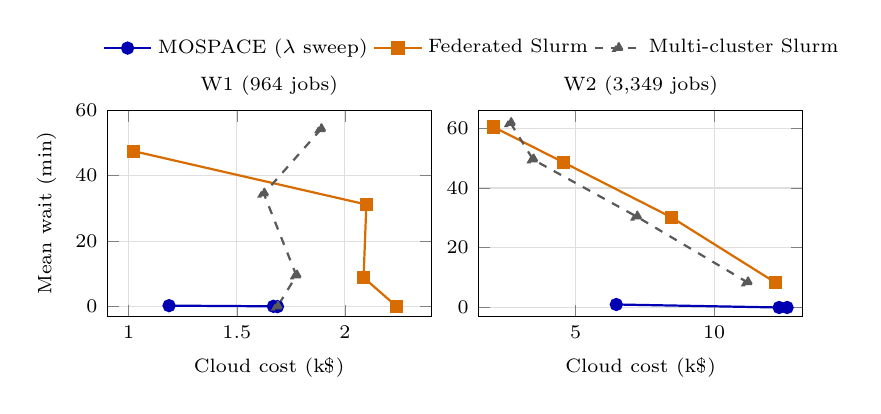
\begin{tikzpicture}
\begin{groupplot}[
  group style={group size=2 by 1, horizontal sep=0.6cm},
  width=0.47\columnwidth, height=4.2cm,
  xlabel={Cloud cost (k\$)}, tick label style={font=\scriptsize},
  label style={font=\scriptsize}, title style={font=\scriptsize, yshift=-1ex},
  ymin=-3, grid=major, grid style={gray!25},
  legend style={font=\scriptsize, at={(1.13,1.2)}, anchor=south, legend columns=3, draw=none},
]
\nextgroupplot[title={W1 (964 jobs)}, ylabel={Mean wait (min)}, xmin=0.9, xmax=2.4, ymax=60]
\addplot[thick, mark=*, color=blue!70!black] coordinates {(1.1866,0.3) (1.6695,0.1) (1.6881,0.0)};
\addplot[thick, mark=square*, color=orange!85!black] coordinates {(1.0234,47.5) (2.0995,31.2) (2.0866,8.9) (2.2404,0.0)};
\addplot[thick, mark=triangle*, color=gray!70!black, dashed] coordinates {(1.8893,54.2) (1.6252,34.5) (1.7757,9.5) (1.6881,0.0)};
\legend{{MOSPACE ($\lambda$ sweep)}, {Federated Slurm}, {Multi-cluster Slurm}}
\nextgroupplot[title={W2 (3,349 jobs)}, xmin=1.5, xmax=13.2, ymax=66]
\addplot[thick, mark=*, color=blue!70!black] coordinates {(6.4712,1.0) (12.3479,0.0) (12.6350,0.0)};
\addplot[thick, mark=square*, color=orange!85!black] coordinates {(2.0423,60.4) (4.5774,48.5) (8.4568,30.2) (12.2219,8.3)};
\addplot[thick, mark=triangle*, color=gray!70!black, dashed] coordinates {(2.6576,61.7) (3.4676,49.5) (7.2112,30.4) (11.2061,8.4)};
\end{groupplot}
\end{tikzpicture}
\caption{Cost--waiting-time trade-off with cloud offloading (data of Table~\ref{tab:cloud-slurm-baselines}). Slurm points are cloud clusters of 50, 100, 200 and 400 nodes.}
\label{fig:tradeoff}
\end{figure}

Fig.~\ref{fig:tradeoff} and Table~\ref{tab:cloud-slurm-baselines} show the effect of adding the cloud. For the Slurm baselines, the operator controls cost only indirectly, through the size of the cloud cluster; for MOSPACE, through $\lambda$. On W1, MOSPACE with $\lambda=0.25$ brings the mean wait down to 0.3\,min for \$1,187. The Slurm configurations need 400 cloud nodes to reach a comparable wait, at \$1,688 (multi-cluster, 42\% more) or \$2,240 (federated, 89\% more); with 50 to 200 nodes they spend between \$1,023 and \$2,100 and still wait 9 to 54\,min on average. On W2, the congestion episode, the difference is larger: MOSPACE with $\lambda=0.25$ keeps the mean wait at 1.0\,min and the bounded slowdown at 1.01 for \$6,471, while the largest Slurm configurations spend \$11,206 and \$12,222 (73\% and 89\% more) and still leave jobs waiting 8.3--8.4\,min on average. On both workloads, every Slurm configuration that spends at least as much as MOSPACE with $\lambda=0.25$ is dominated by a MOSPACE configuration (on W1, multi-cluster Slurm with 400 nodes ties with $\lambda=0.75$). MOSPACE achieves this by choosing \emph{which} jobs to offload: on W2 at $\lambda=0.25$ it offloads 1,667 jobs, more than any Slurm configuration, but selects those whose cloud execution is cheap relative to the waiting time it saves, while Slurm offloads whichever job finds the cloud cluster free. Increasing $\lambda$ beyond 0.25 removes the last minute of waiting but almost doubles the cost on W2, which illustrates how the single parameter exposes the trade-off to the operator.

\subsection{Planner speed and quality}

\begin{table}[t]
\centering\footnotesize
\setlength{\tabcolsep}{4pt}
\caption{Gurobi versus the GA on the 108 benchmark instances. Each row averages 27 runs (9 instances $\times$ 3 values of $\lambda$); GA values average 3 seeds. Gurobi solved every run to optimality. Gap: GA objective above the optimum (\%). \#Opt: runs in which the GA found the optimum. $t$: mean wall-clock time (s).}
\label{tab:ga-vs-gurobi}
\begin{tabular}{llrrrrr}
\toprule
 & & & Gurobi & \multicolumn{3}{c}{GA} \\
\cmidrule(lr){4-4}\cmidrule(lr){5-7}
Class & Wkl. & $N$ & $t$ & Gap & \#Opt & $t$ \\
\midrule
\multirow{6}{*}{A} & \multirow{3}{*}{W1} & 100 & 19.7 & 0.84 & 5 & 2.0 \\
 & & 300 & 12.9 & 0.53 & 19 & 1.4 \\
 & & 500 & 9.5 & 0.02 & 24 & 1.1 \\
\cmidrule(lr){2-7}
 & \multirow{3}{*}{W2} & 100 & 216.9 & 16.59 & 0 & 15.4 \\
 & & 300 & 92.1 & 5.53 & 0 & 9.2 \\
 & & 500 & 73.9 & 4.28 & 6 & 7.1 \\
\midrule
\multirow{6}{*}{B} & \multirow{3}{*}{W1} & 100 & 29.8 & 0.99 & 0 & 2.1 \\
 & & 300 & 20.6 & 0.33 & 16 & 1.5 \\
 & & 500 & 15.3 & 0.07 & 18 & 1.2 \\
\cmidrule(lr){2-7}
 & \multirow{3}{*}{W2} & 100 & 303.9 & 17.34 & 0 & 12.8 \\
 & & 300 & 196.0 & 4.09 & 3 & 7.5 \\
 & & 500 & 101.9 & 1.70 & 12 & 5.5 \\
\midrule
\multicolumn{3}{l}{All} & 91.1 & 4.36 & 103 & 5.6 \\
\bottomrule
\end{tabular}
\end{table}

Table~\ref{tab:ga-vs-gurobi} shows that the arc-flow MILP is solved to optimality on all 108 instances and three values of $\lambda$, in 91\,s on average. The hardest configurations (W2 with $N=100$) average 217--304\,s, above the 180\,s online budget, in which case the online planner would stop with the best incumbent found. Instances get harder when on-premises capacity is scarce ($N=100$) and on W2, whose larger jobs and long tail make the choice of which jobs to offload more consequential. The GA is 16 times faster on average (5.6\,s) and within 4.36\% of the optimum. On W1 its gap is below 1\% in every configuration; on W2 with $N=100$, the most congested setting, it reaches 17\%, so the MILP remains preferable when a solver license is available and the event rate allows it. The GA is a practical fallback for sites without a commercial solver or with higher event rates.

% =====================================================================
\section{Conclusion}
\label{sec:conclusion}
% =====================================================================

We presented MOSPACE, a central scheduler that re-plans, at every submission and completion event, the placement and start time of all pending parallel jobs of a federation of HPC clusters and cloud instance pools, balancing priority-weighted turnaround against monetary cost through a single operator-chosen weight. Planning relies on an arc-flow MILP, solved to optimality in about a minute, or on a memetic GA that returns plans within a few percent of the optimum in seconds. In Batsim simulations of a production cluster of Petrobras driven by its own Slurm logs, MOSPACE reduced the mean waiting time by 20--49\% relative to Slurm's multi-cluster and federated modes without cloud resources and, with cloud bursting, reached near-zero waiting for 30--47\% less money than the Slurm configurations that came closest. Hence, even when a federation-capable RJMS is in place, there is substantial room for cost-aware, federation-level scheduling.

The current work has limitations that point to future work. MOSPACE assumes known runtimes; we plan to couple it with the runtime predictor available for this cluster~\cite{Nunes2025} and to measure its sensitivity to prediction errors. The experiments simulate a single on-premises site with one cloud provider; multi-site federations with real inter-site data movement and multi-cloud pricing remain to be evaluated. The weighted-turnaround objective lengthens the tail of the waiting-time distribution, which calls for fairness terms. Finally, the central scheduler should be integrated with production RJMS, for instance by submitting its decisions to the member clusters' Slurm instances.

\bibliographystyle{IEEEtran}
\bibliography{bibliography}
\end{document}
